%!TEX root = emnlp2016.tex

In this section, we present the Capsule model for detecting and
characterizing significant diplomatic events. We first provide the
intuition behind Capsule, and then formally specify the model. We also
explain how to use Capsule to explore a corpus and how to learn the
posterior distribution of the latent variables.

\begin{figure}
\centering
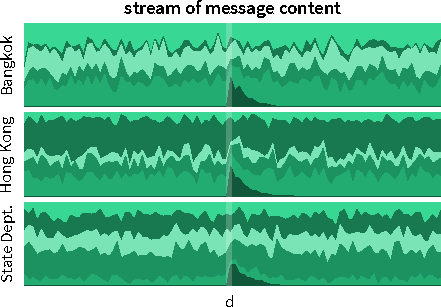
\includegraphics[width=\linewidth]{fig/cartoon.pdf}
\caption{Cartoon intuition. The $y$-axis represents the stacked
  proportions of cables about various topics, while the $x$-axis
  represents time. The Bangkok embassy, Honk Kong embassy, and
  U.S. State Department all have typical diplomatic business, about
  which they usually send cables. When an event occurs during time
  interval $t$, the cables alter to cover the event before returning
  to ``business as usual.'' Capsule discovers the embassies' typical
  concerns, as well as the timing and content of events.}
\label{fig:cartoon}
\end{figure}

Consider an entity like the Bangkok embassy, as illustrated in
\cref{fig:cartoon}. We can imagine that this entity sends a stream of
diplomatic cables over time---some to the U.S. State Department,
others to other American embassies, such as the one in Hong
Kong. Embassies usually write cables that describe typical diplomatic
business. For example, the Bangkok embassy might write about topics
regarding southeast Asia more generally. We can think of a topic as
being a probability distribution over vocabulary terms.

Now imagine that an event, such as the capture of Saigon during the
Vietnam War, occurs during a particular time interval $t$. We cannot
directly observe the occurrence of this event, but we can observe the
stream of cables and the event's impact on it. When the event occurs,
multiple entities deviate from their usual topics of discussion
simultaneously, before returning to their usual behavior, as depicted
in \cref{fig:cartoon}. For example, the day after the capture of
Saigon, the majority of the diplomatic cables written by the Bangkok
embassy and several other entities were about Vietnam War refugees. If
we think of the event as another probability distribution over
vocabulary terms, then each entity's stream of cables reflects its
typical concerns, as well as any significant events.


% \parhead{Background: Topic Models.} Capsule builds on topic models.  Topic models are algorithms for discovering the main themes in a large collection of documents; each document can then be summarized in terms of the global themes.  More formally, a topic $k$ is a probability distribution over the set of vocabulary words.  Each document $d$ is represented as a distribution over topics $\theta_d$.  Thus we can imagine that when we generate a document, we first pick which topics are relevant (and in what proportions).  Under the LDA topic model~\cite{Blei:2003}, we know the number of words in each document.  Then, for each word, we select a single topic from this distribution over topics, and finally select a vocabulary term from the corresponding topic's distribution over the vocabulary.  Alternatively, we can cast topic modeling as factorization, such as in Poisson factorization~\cite{Gopalan:2014b}, and draw a word count for each term in the vocabulary.

% Topic models are often applied to provide a structure for an
% otherwise unstructured collection of documents.  Documents, however,
% are often accompanied by metadata, such as the date written or
% author attribution; this information is not exploited by traditional
% topic models.  The Capsule model uses both author and date
% information to identify and characterize events that influence the
% content of the collection.

\subsection{Model Specification}
\label{sec:model_spec}

We now define the Capsule model. Our data come from \emph{entities}
(e.g., embassies) who send \emph{messages} (e.g., diplomatic cables)
over \emph{time}; specifically, we observe the number of times
$n_{dv}$ that each vocabulary term $v$ occurs in each message
$d$. Each message is associated with an author entity $a_d$ and a time
interval $t_d$ within which that message was sent.

We model each message with a bank of Poisson distributions\footnote{Readers familiar with topic modeling may expect a multinomial model of word tokens, but Poisson models of word counts better capture documents of different lengths \cite{canny2004gap}.}---one for
each vocabulary term:
\begin{align}
  n_{dv} \sim \textrm{Poisson}\left(\lambda_{dv}\right).
\end{align}
The rate $\lambda_{dv}$ blends the different influences on message
content. Specifically, it blends three types of \emph{topics},
intended to capture ``business-as-usual'' discussion and content
related to significant events.

We operationalize each topic as a specialized probability distribution
over vocabulary terms (the set of unique words in the corpus of
messages), as is common in topic
models~\cite{Blei:2003,canny2004gap,Gopalan:2014b}---i.e., each term
is associated with each topic, but with a different probability.

\begin{table}
\centering
\small
\begin{tabular}{cc}
\toprule
\textbf{Topic Type} & \textbf{Top Terms} \\
\midrule
General & visit, hotel, schedule, arrival \\
Entity & soviet, moscow, ussr, agreement \\
Event & saigon, evacuation, vietnam, help \\
\bottomrule
\end{tabular}
\caption{The highest-probability vocabulary terms for examples of the
  three types of topics (general, entity, and event). These examples
  come from the analysis that we describe \cref{sec:eval}.}
\label{tab:3topics}
\end{table}

Each message blends 1) general topics $\mathbold{\beta}_1, \ldots,
\mathbold{\beta}_K$ about diplomacy (e.g., terms about diplomats,
terms about communication), 2) an entity topic $\mathbold{\eta}_{a_d}$
specific to the author of that message (e.g., terms about
Hong Kong),\footnote{The entity-specific topics play a similar role to the
  background topics introduced by Paul and
  Dredze~\shortcite{paul2012model}.} and 3) event topics
$\mathbold{\gamma}_1, \ldots, \mathbold{\gamma}_T$ that are specific
to the events in recent time intervals (e.g., terms about a coup,
terms about the death of a dignitary).

Examples of these three types of topics are in \cref{tab:3topics}. The
general topic relates to planning travel, the entity topic captures
words related to the U.S.S.R., and the event topic captures words
related to the evacuation of Saigon toward the end of the Vietnam War.

The messages share the three types of topics in different ways: all
messages share the general topics, messages written by a single entity
share an entity topic, and messages in the same time interval use the
event topics in similar ways. Each message blends its corresponding
topics with a set of message-specific strengths. As a result, each
message captures a different mix of general diplomacy discussion,
entity-specific terms, and recent events. Specifically, the Poisson
rate for vocabulary term $v$ in message $d$ is
\begin{align}
  \lambda_{dv} &= \sum_{k=1}^K \theta_{dk} \beta_{kv}  + \zeta_d
  \eta_{a_dv} + {}\notag \\
  &\quad
  \sum_{t=1}^T f(t_d, t)\, \epsilon_{dt} \gamma_{tv},
\label{eq:poisrate}
\end{align}
where $\theta_{dk}$ is message $d$'s strength for general topic $k$,
$\zeta_{d}$ is message $d$'s strength for $a_d$'s entity topic, and
$\epsilon_{dt}$ is message $d$'s strength for event topic $t$. The
function $f(\cdot)$ ensures that the events influences decay over
time. As we describe in \cref{sec:additional_results}, we compared
several different decay functions (exponential, linear, and step) and
found that the following exponential decay function works well in
practice:
\begin{equation}
  f(t_d, t) = \begin{cases}
    0 & \textrm{$t \le t_d < t + \tau$}\\
    \exp{\left( \frac{-(t_d - t)}{\tau\,/\,5}\right)} &
    \textrm{otherwise.}
    \end{cases}
  \label{eq:f}
  \end{equation}
Dividing $\tau$ by five means that we can interpret it as the number
of time intervals after which an event will have little impact on the
content of the messages.

We place hierarchical gamma priors over the message-specific
strengths, introducing entity-specific strengths $\mathbold{\phi}_1,
\ldots, \mathbold{\phi}_A$ and $\xi_1, \ldots, \xi_A$ that allow
different entities to focus on different topics and event strengths
$\psi_1, \ldots, \psi_T$ that allow different time intervals to be
more or less ``eventful.'' We place Dirichlet priors over the
topics. The graphical model is in \cref{fig:graphicalmodel} and the
generative process is in \cref{fig:generative-model}.

% NEED TO REMAKE THIS to use A rathre than N and n rather than w
\begin{figure}[bt]
\centering
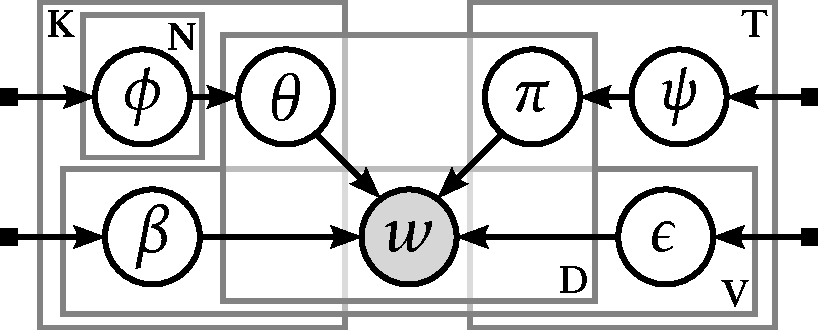
\includegraphics[width=0.6\linewidth]{fig/graphicalmodel.pdf}
\caption{Graphical model for Capsule. Observed term counts depend on
  general topics $\mathbold{\beta}_1, \ldots, \mathbold{\beta}_K$,
  entity topics $\mathbold{\eta}_1, \ldots, \mathbold{\eta}_A$, and
  event topics $\mathbold{\gamma}_1, \ldots, \mathbold{\gamma}_T$, as
  well as message-specific strengths $\mathbold{\theta}_d$, $\zeta_d$,
  and $\mathbold{\epsilon}_d$.  Variables $\mathbold{\phi}_1, \ldots,
  \mathbold{\phi}_A$ and $\xi_1, \ldots, \xi_A$ represent
  entity-specific strengths, while $\psi_1, \ldots, \psi_T$ allow time
  intervals to be more or less ``eventful.'' Black squares denote
  hyperparameters (unlabeled for visual simplicity).}
\label{fig:graphicalmodel}
\end{figure}

\begin{figure}[!ht]
\begin{mdframed}[userdefinedwidth=3.0in,align=center]
\small
\begin{itemize}[leftmargin=*]
\item for $k= 1, \ldots, K$,
	\begin{itemize}[leftmargin=*]
	\item draw general topic\\ $\mathbold{\beta}_k \sim
          \textrm{Dirichlet}_V (\alpha, \ldots, \alpha)$
	\item for each entity $a=1, \ldots, A$,
		\begin{itemize}[leftmargin=*]
		\item draw entity-specific strength \\$\phi_{ak} \sim \textrm{Gamma}\,(s, r)$
		\end{itemize}
                \end{itemize}
\item for each entity $a = 1, \ldots, A$,
	\begin{itemize}[leftmargin=*]
	\item draw entity topic \\$\mathbold{\eta}_a \sim
          \textrm{Dirichlet}_V (\alpha, \ldots, \alpha)$
	\item draw entity-specific strength \\$\xi_{a} \sim \textrm{Gamma}\,(s, r)$
	\end{itemize}
\item for each time interval $t = 1, \ldots, T$,
	\begin{itemize}[leftmargin=*]
	\item draw event topic\\ $\mathbold{\gamma}_t \sim
          \textrm{Dirichlet}_V(\alpha, \ldots, \alpha)$
	\item draw event strength \\$\psi_{t} \sim \textrm{Gamma}\,(s, r)$
	\end{itemize}
\item for each message $d= 1, \ldots, D$, sent during time interval
  $t_d$ by author entity $a_d$,
	\begin{itemize}[leftmargin=*]
	\item for each general topic $k = 1, \ldots, K$,
		\begin{itemize}[leftmargin=*]
			\item draw message-specific strength
                          \\$\theta_{dk} \sim \textrm{Gamma}\,(s,
                          \phi_{a_d k})$
		\end{itemize}
	\item draw message-specific strength \\$\zeta_{d} \sim \textrm{Gamma}\,(s, \xi_{a_d})$
	\item for each time interval $t=1, \ldots, T$,
		\begin{itemize}[leftmargin=*]
			\item draw message-specific strength \\$\epsilon_{dt} \sim \textrm{Gamma}\,(s, \psi_{t})$
		\end{itemize}
	\item for each vocabulary term $v=1, \ldots, V$,
		\begin{itemize}[leftmargin=*]
			\item set $\lambda_{dv} = \sum_{k=1}^K
                          \theta_{dk} \beta_{kv}  + \zeta_d \eta_{a_d
                            v} + {}$\\$ \sum_{t=1}^T f(t_d, t)\, \epsilon_{dt} \gamma_{tv}$
			\item draw term counts \\$n_{d,v} \sim \textrm{Poisson}\left(\lambda_{dv}\right)$
		\end{itemize}
	\end{itemize}
\end{itemize}
\end{mdframed}
\caption{Generative process for Capsule. We use $s$ and $r$ to denote
  top-level (i.e., fixed) shape and rate hyperparameters; they can be
  set to different values for different variables.}
\label{fig:generative-model}
\end{figure}

Given a corpus of messages, learning the posterior distribution of the
latent variables uncovers the three types of topics, the message- and
entity-specific strengths, and the event strengths. In
\cref{sec:detecting}, we explain how an analyst can use the event
strengths as a filter that isolates potentially significant messages.

\subsection{Learning the Posterior Distribution}

In order to use Capsule to to explore a corpus of messages, we must
first learn the posterior distribution of the latent variables---the
general topics, the entity topics, the event topics, the message- and
entity-specific strengths, and the event strengths---conditioned on
the observed term counts. As for many Bayesian models, this posterior
distribution is not tractable to compute; approximating it is
therefore our central statistical and computational problem. We
introduce an approximate inference algorithm for Capsule, based on
variational methods~\cite{Jordan:1999},\footnote{Source code:
  \url{https://github.com/ajbc/capsule}.}, which we outline in
\cref{sec:inference}.\footnote{Appendices are in the supplemental
  material.} This algorithm produces a fitted variational distribution
which be can then be used as a proxy for the true posterior
distribution.

\subsection{Detecting and Characterizing Events}
\label{sec:detecting}

We can use the mean of the fitted variational distribution to explore
the data. Specifically, we can explore ``business-as-usual'' content
using the posterior expected values of the general topics
$\mathbold{\beta}_1, \ldots, \mathbold{\beta}_K$ and the entity topics
$\mathbold{\eta}_1, \ldots, \mathbold{\eta}_A$, and we can detect and
characterize events using the posterior expected values of the event
strengths and the event topics.

To detect events, we define an measure that quantifies the
``eventness'' of time interval $t$. Specifically, we first compute how
relevant each message $d$ is to that time interval: $m_{dt} = f(t_d,
t)\,\E[\epsilon_{dt}]$. Using these relevancy values, we then compute
the proportion of each message's term counts that are associated with
the event topic specific to time interval $t$:
\begin{equation}
  p_{dt}= \frac{m_{dt}}{\sum_{k}
    \E[\theta_{dk}] + \E[\zeta_d] +
    \sum_{t'} m_{dt'}}.
\end{equation}
Finally, we aggregate these values over messages:
\begin{equation}
  \frac{1}{\sum_{d} f(t_d, t)}\sum_{d=1}^D p_{dt},
  \label{eq:eventness}
\end{equation}
where the multiplicative fraction ensures that messages that were sent
during time intervals that are further from $t$ contribute less than
than messages that were sent during time intervals that are closer to
$t$.

We can characterize an event $t$ by selecting the highest-probability
vocabulary terms from $\E[\mathbold{\gamma}_t]$. By ordering the
messages according to $m_{dt} = f(t_d, t)\,\E[\epsilon_{dt}]$, we can
also identify the messages that are most strongly associated with
event $t$.

In \cref{sec:eval}, we explore the cables associated with
significant events in the National Archives' corpus of diplomatic
cables. To make Capsule more accessible for historians, political
scientists, and journalists, we have released an open-source tool for
visualizing its results.\footnote{Source code:
  \url{https://github.com/ajbc/capsule-viz}; demo:
  \url{http://www.princeton.edu/~achaney/capsule/}.} This tool allows
analysts to browse a corpus of messages and the mean of the
corresponding posterior distribution, including general topics, entity
topics, and event topics. \Cref{fig:viz} contains several screenshots
of the tool's browsing interface.

\begin{figure}
\centering
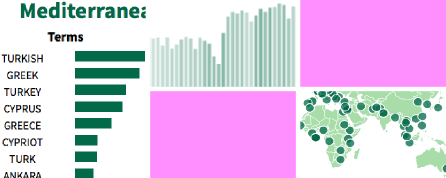
\includegraphics[width=\linewidth]{fig/viz.png}
\caption{Screenshots of the Capsule visualization tool used to explore
  U.S. State Department cables. Top left: events over time (similar to
  \cref{fig:cables_events}). Top right: entities located on a
  map. Bottom: summary of the week of May 12, 1975, including top
  vocabulary terms, relevant cables, and text from Wikipedia.}
\label{fig:viz}
\end{figure}
